% KSN - wzór sprawozdania
% kodowanie polskich znaków: ISO-8859-2

\documentclass[10pt,a4paper]{article}
\usepackage[margin=2cm]{geometry}
\usepackage{graphicx}
\usepackage[utf8]{inputenc}
\usepackage[polish]{babel}
\usepackage{polski}
\usepackage{amsmath}
\usepackage{mathtools}
\usepackage{subcaption}
\usepackage{float}
\author{Ryniak}

\begin{document}

% =====  STRONA TYTULOWA PRACY INŻYNIERSKIEJ ====
% ostatnia modyfikacja: 2011/03/09, K. Malarz

\thispagestyle{empty}
\vspace*{50ex}
\begin{center}
{\bf\LARGE\textsf{Sprawozdanie do projeku:}}\\
\vspace{5ex}

{\bf\huge\textsf{Wykorzystanie probabilistycznych sieci neuronowych do klasyfikacji danych o zmiennym harakterze}}\\
\vspace{54ex}

{\bf\Large\textsf{Grzegorz Ryniak, Rafał Szęszoł}}\\
\vspace{22ex}
\textsf{\bf\large\textsf{Kraków, czerwiec 2018}}
\end{center}


\newpage

\section{Wstęp}
W świecie rzeczywistym często spotykamy się ze źródłami informacji, które z czasem zaczynają przesyłać zmodyfikowane dane. Przykładem może być elektroniczny czujnik grubości - odpowiednik czujnika zegarkowego. W skutek zużycia np. końcówek pomiarowych, z czasem otrzymywane wartości mogą być zaniżone. Duży problem pojawia się kiedy odbierane dane poddawane są klasyfikacji. Klasyfikator widząc przesunięcie danych może uznać, że należą one do innej klasy. Z czasem tych klas mogło by powstać coraz więcej. Ze względu na ograniczone zasoby i łatwość interpretacji często wymaga się, aby liczba klas była stała. Celem tego projektu było stworzenie klasyfikatora opartego o probabilistyczne sieci neuronowe, który byłby w stanie na bieżąco dostosowywać się do zmiennych danych. 

\section{Doświadczenia}
Wszystkie symulacje zostały przeprowadzone z wykorzystaniem środowiska MATLAB 2012b. W pierwszej kolejności stworzono generator danych, który symulował by rzeczywiste źródło informacji podlegające zużyciu. Generowane były 2 klasy dwu-wymiarowych danych. Dane takie łatwo da się przedstawić na układzie współrzędnych w postaci punktów. Pierwsza klasa składała się z punktów o współrzędnych generowanych z rozkładu Gaussa o średniej wartości (0;0) i odchyleniu 1, natomiast druga klasa również była generowana na podstawie rozkładu Gaussa o średnim odchyleniu 1 ale średnie wartości były punktami leżącymi na okręgu o promieniu 2 i środku w punkcie (0;0). Kąt pomiędzy osią x a promieniem zwiększał się z czasem w kierunku przeciwnym do wskazówek zegara. Co 90 stopni ruch na chwilę się zatrzymywał, aby sprawdzić, czy sieć nie przyzwyczaiła się do ruchu. Generowanie danych kończy się w momencie kiedy druga klasa ,,okrąży'' pierwszą dookoła. Kolejne etapy generowania danych pokazane są na rysunku \ref{dataGen}. 
\begin{figure}[h]
  \begin{subfigure}[b]{0.4\textwidth}
    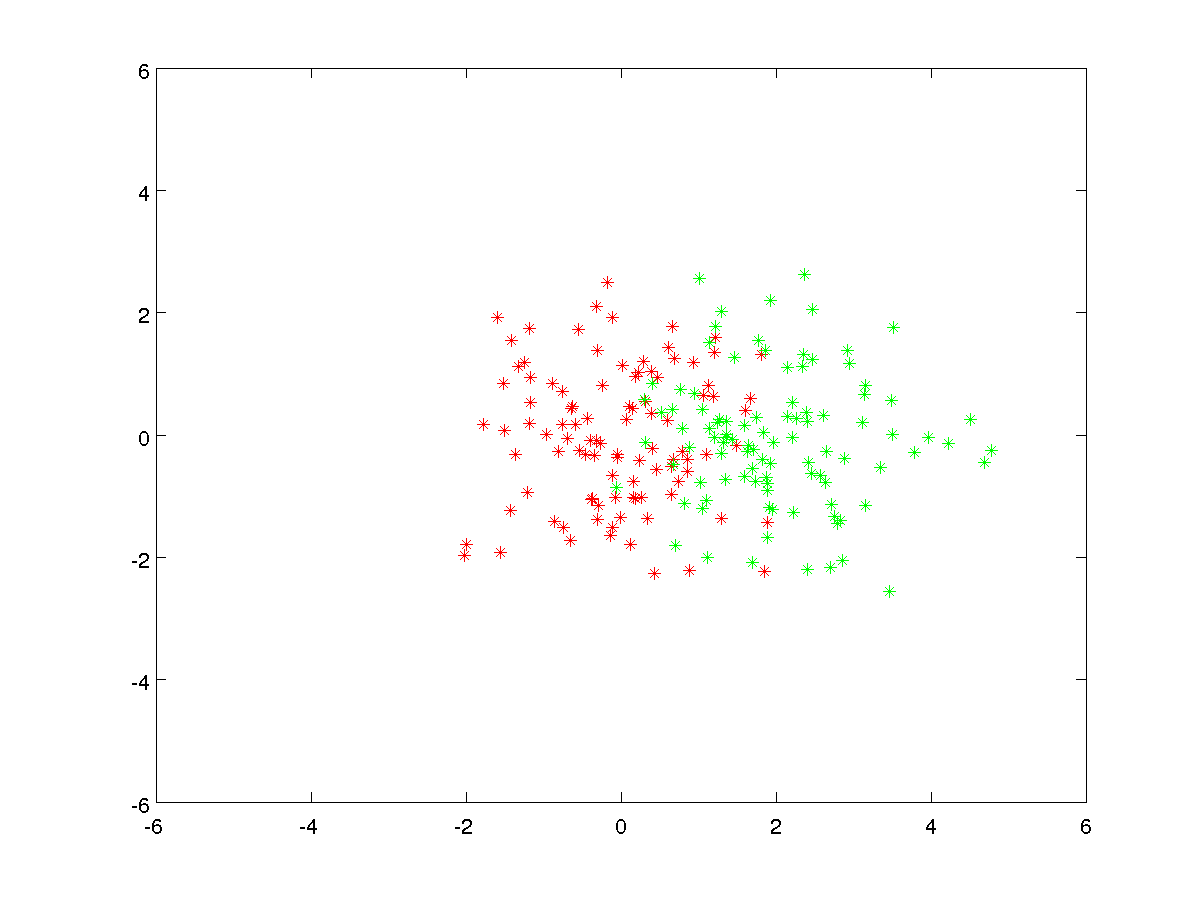
\includegraphics[width=\textwidth]{dataGen_step0.png}
    \caption{Krok 1}
  \end{subfigure}
  \hfill
  \begin{subfigure}[b]{0.4\textwidth}
    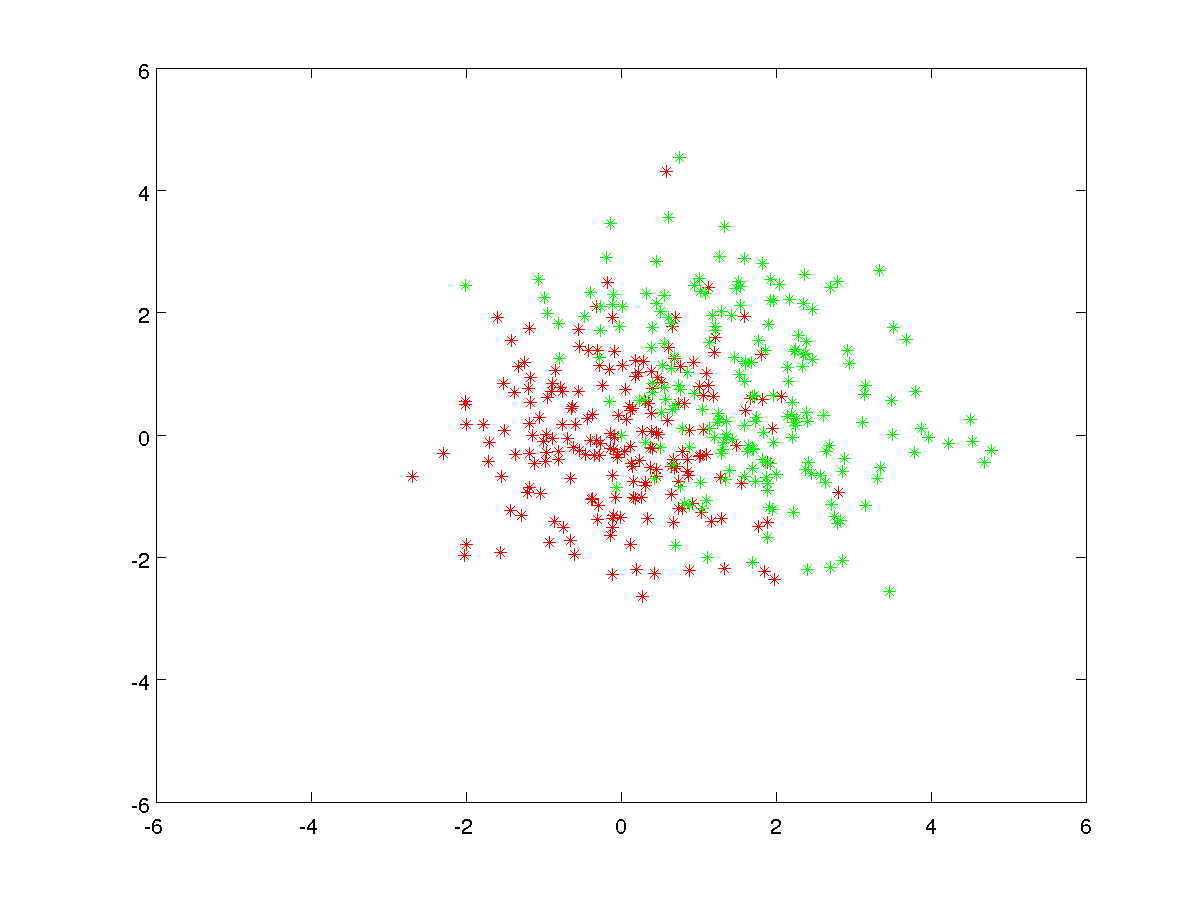
\includegraphics[width=\textwidth]{dataGen_step1.png}
    \caption{Krok 2}
  \end{subfigure}

   \begin{subfigure}[b]{0.4\textwidth}
    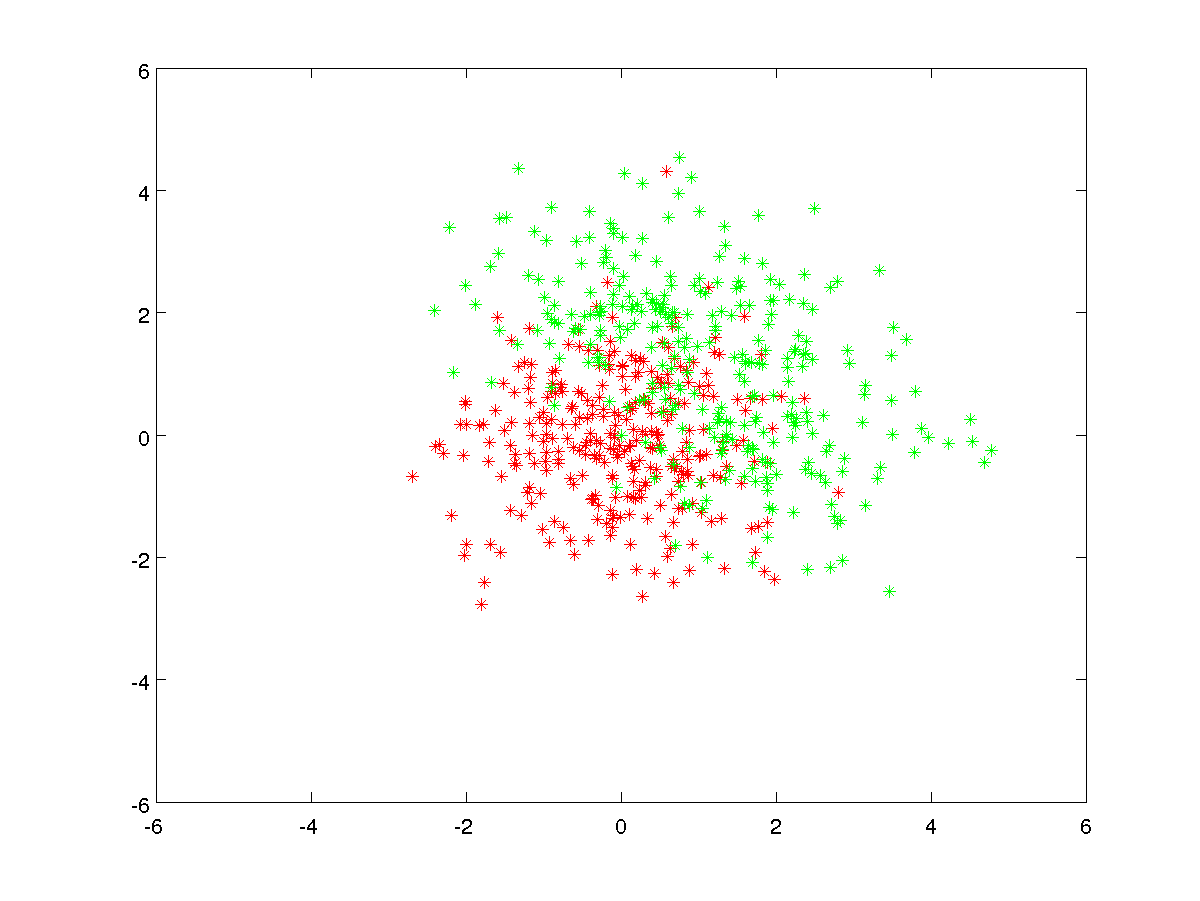
\includegraphics[width=\textwidth]{dataGen_step2.png}
    \caption{Krok 3}
  \end{subfigure}
  \hfill
  \begin{subfigure}[b]{0.4\textwidth}
    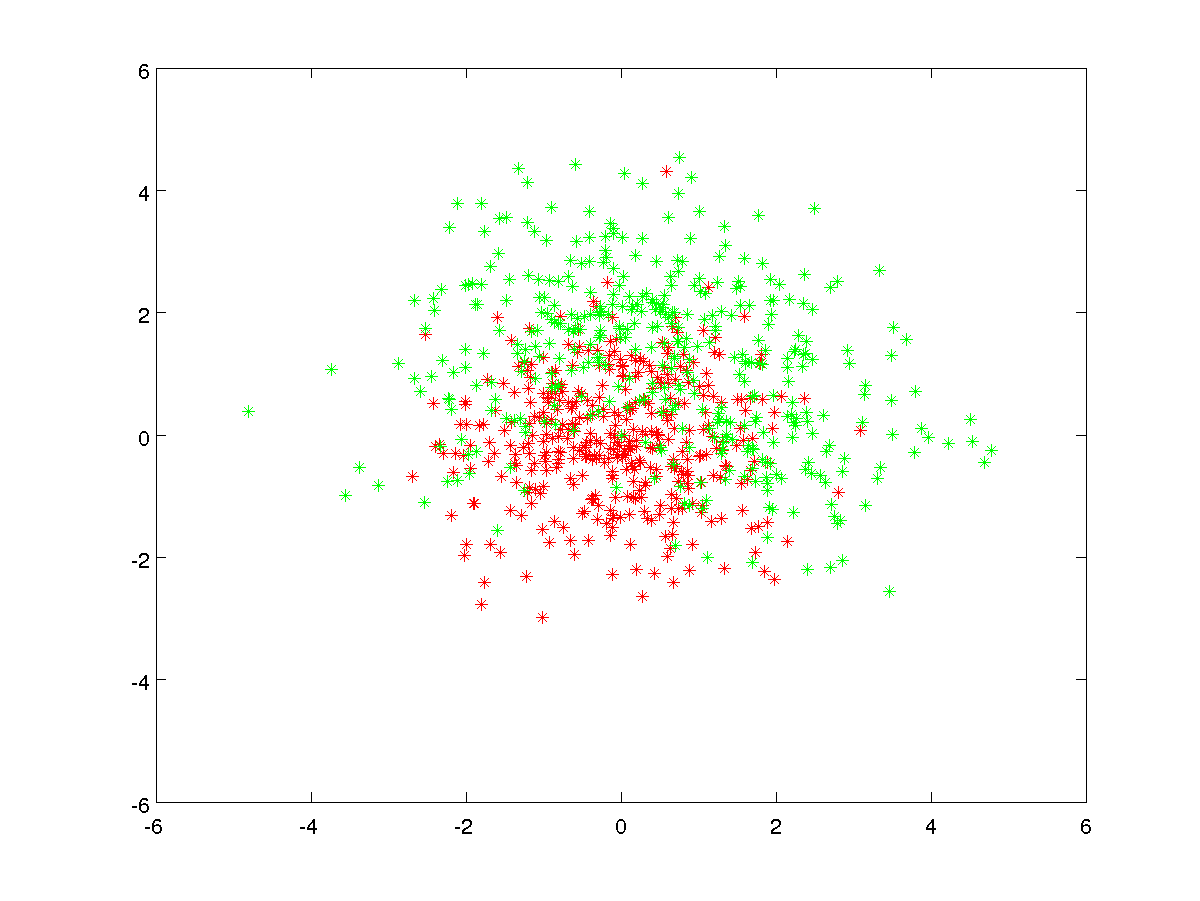
\includegraphics[width=\textwidth]{dataGen_step3.png}
    \caption{Krok 4}
  \end{subfigure}
  
  \begin{subfigure}[b]{0.4\textwidth}
    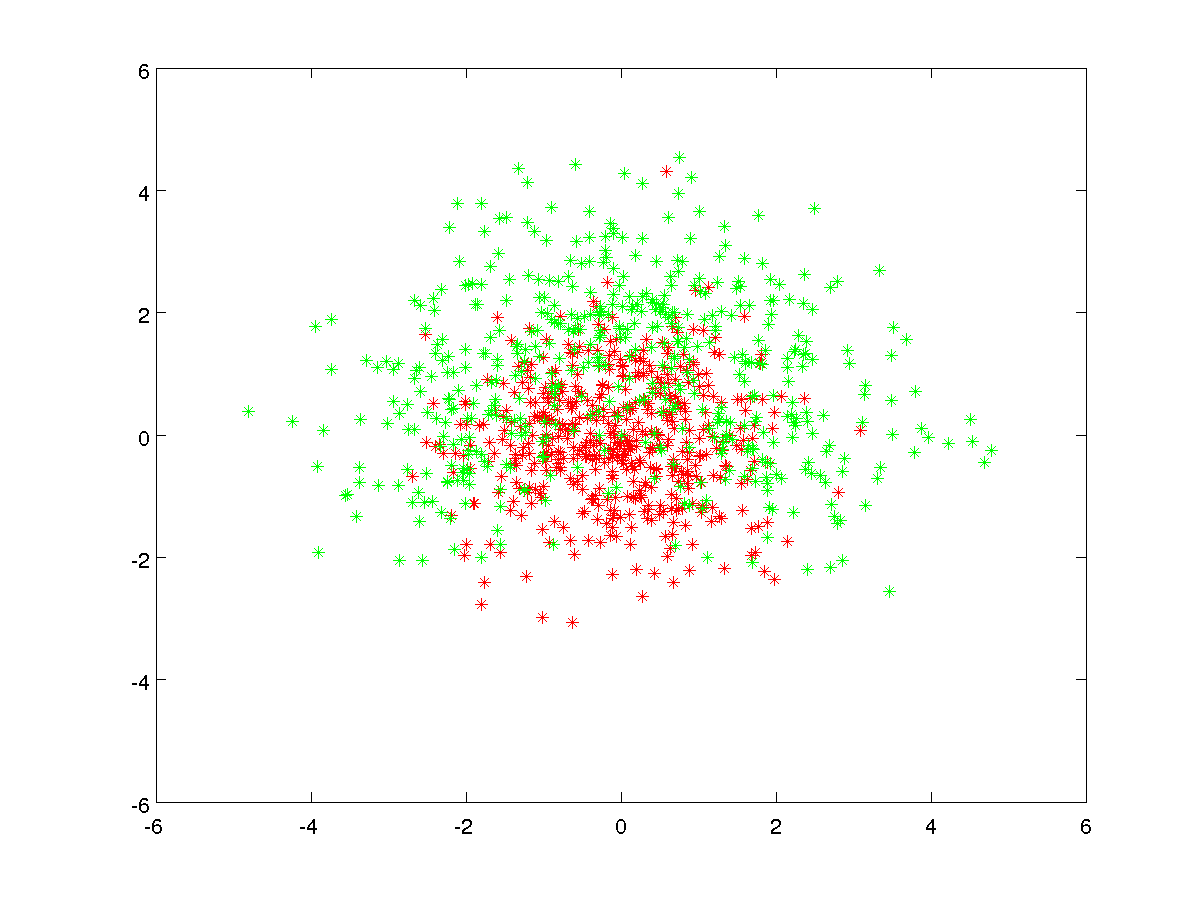
\includegraphics[width=\textwidth]{dataGen_step4.png}
    \caption{Krok 5}
  \end{subfigure}
  \hfill
  \begin{subfigure}[b]{0.4\textwidth}
    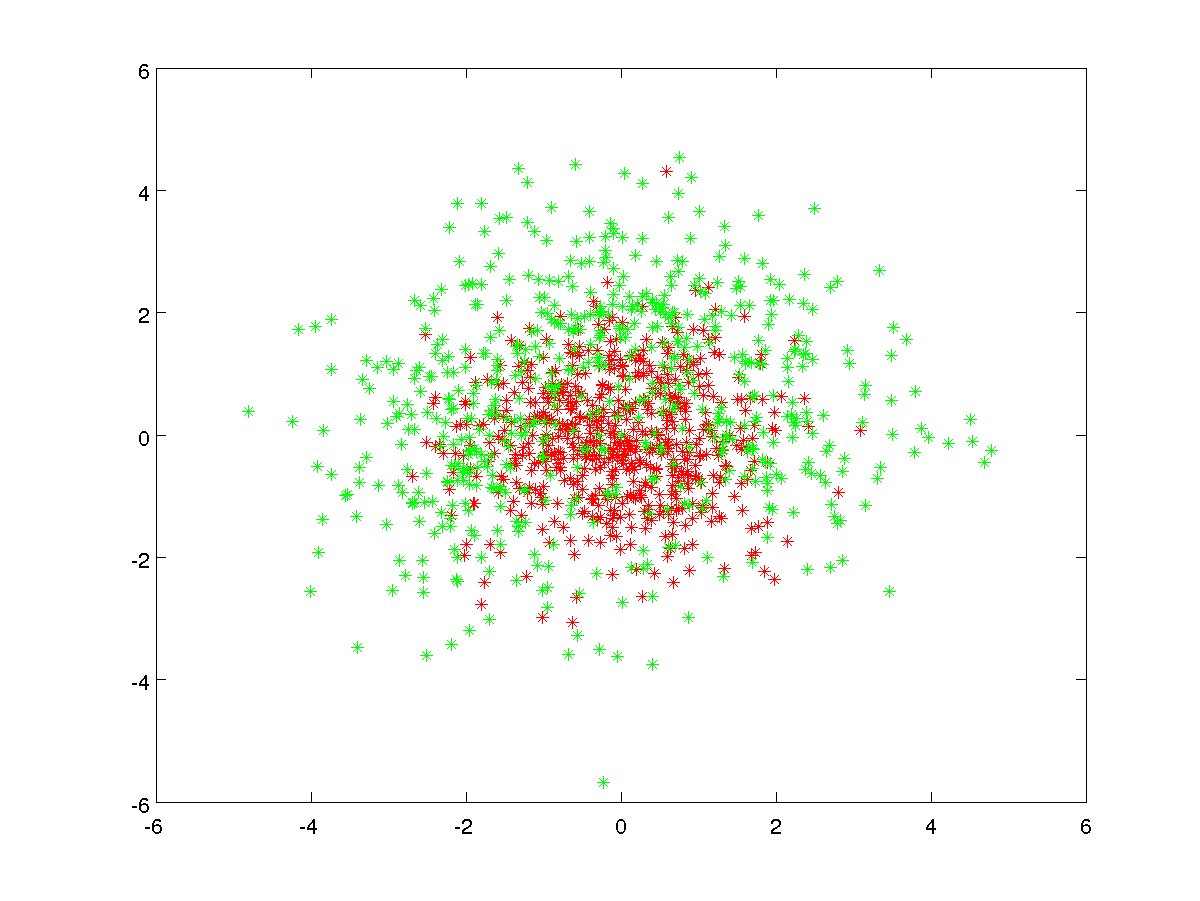
\includegraphics[width=\textwidth]{dataGen_step5.png}
    \caption{Krok 6}
  \end{subfigure}
  
  \begin{center}
  \begin{subfigure}[b]{0.4\textwidth}
    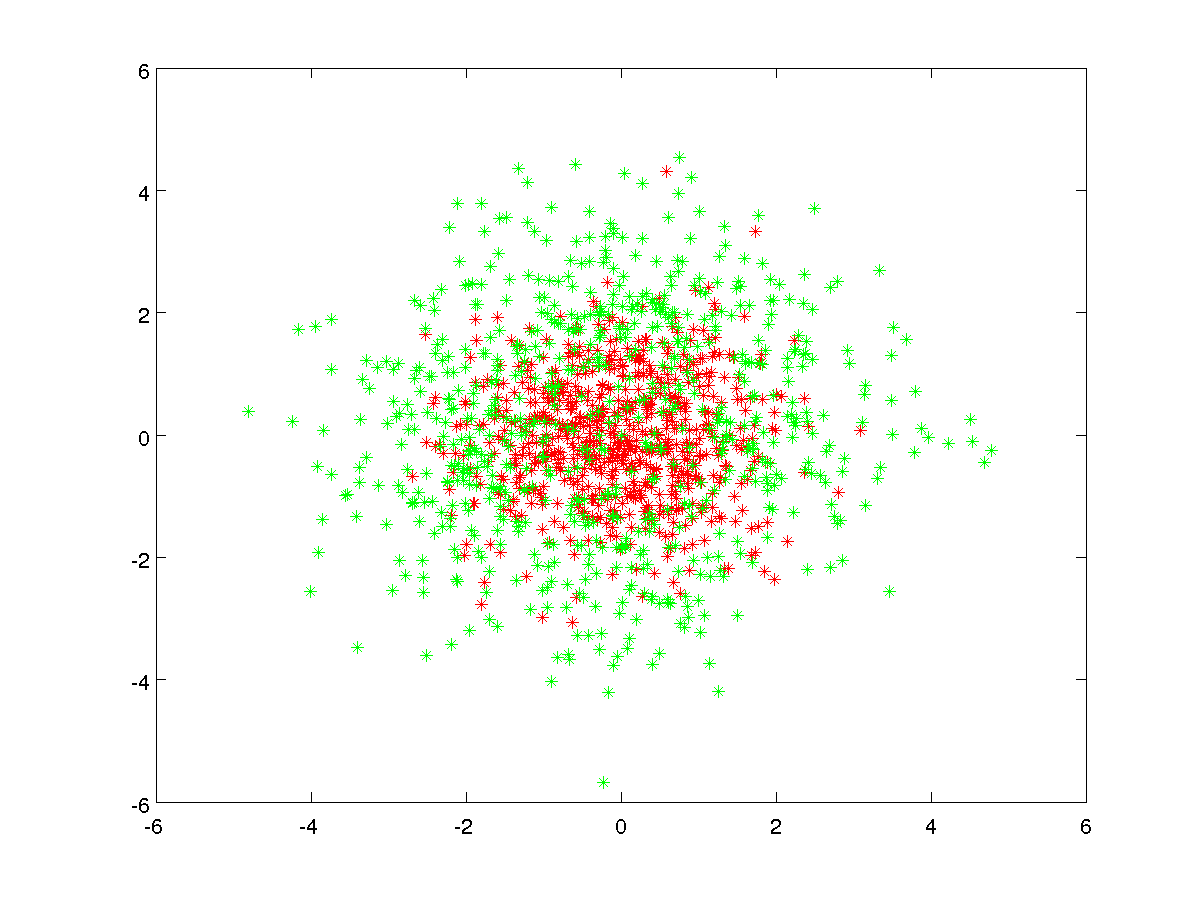
\includegraphics[width=\textwidth]{dataGen_step6.png}
    \caption{Krok 7}
  \end{subfigure}
  \end{center}
  
  \caption{Poszczególne etapy generowania danych}
  \label{dataGen}
  
\end{figure}
Liczbę punktów generowanych w każdym kroku można było zmieniać. Co określoną ilość dodanych punktów sieć neuronowa była uczona nowych danych. Stare punkty były odrzucane wg. 2 metod. Pierwsza metoda polegała na odrzucaniu najstarszych punktów. Punkty były ustawiane w kolejce. Kiedy do kolejki wchodził nowy punkt, najstarszy zostawał z niej usuwany. Długość kolejki mogła być regulowana. Podczas ponownego uczenia sieci, zmianom podlegał parametr wygładzania. Algorytm wyznaczania tegoż parametru został dostarczony przez prowadzącego zajęcia. Podczas symulacji wykonywany był wykres jak w czasie zmienia się procent błędnie sklasyfikowanych punktów oraz mapa, gdzie te punkty się znajdowały. 

Na początku przeprowadzono testy dla stałej wartości spread. Liczbę wszystkich generowanych punktów ustawiono na 8000, natomiast aktualizacja sieci odbywała się co 50 punktów. Rozmiar okna wynosił 1000 punktów. Symulacje przeprowadzono dla h równego 0,0001; 0,001; 0,01; 0,1 oraz 1. Dla każdego testu sporządzony został mapa w błędnymi punktami w ostatniej fazie, wykres zależności błędu od czasu oraz średnia wartość błędu. Wartość błędu była ułamkiem wyrażonym w procentach oznaczającym ilość błędnych klasyfikacji w obrębie całego okna na ilość dodanych nowych punktów, zatem wartość ta może przekroczyć 100 \%. Wyniki przedstawia rysunek \ref{test_h}

\begin{figure}[h]
  \begin{subfigure}[b]{0.5\textwidth}
    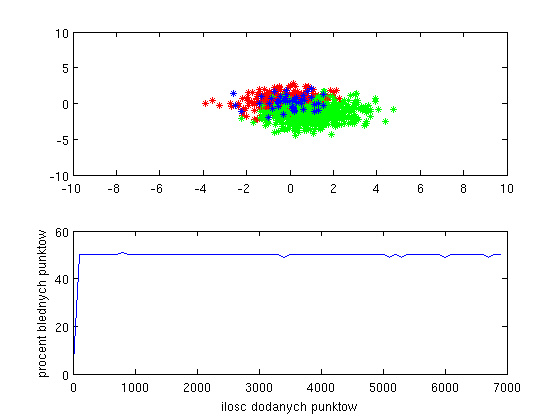
\includegraphics[width=\textwidth]{test_h0_0001.png}
    \caption{h = 0,0001}
  \end{subfigure}
  \hfill
  \begin{subfigure}[b]{0.5\textwidth}
    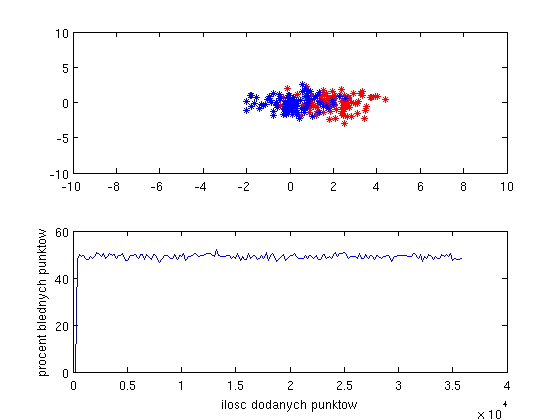
\includegraphics[width=\textwidth]{test_h0_001.png}
    \caption{h = 0,001}
  \end{subfigure}

   \begin{subfigure}[b]{0.5\textwidth}
    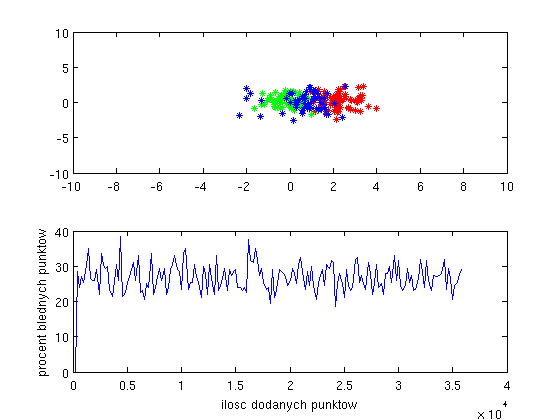
\includegraphics[width=\textwidth]{test_h0_01.png}
    \caption{h = 0,01}
  \end{subfigure}
  \hfill
  \begin{subfigure}[b]{0.5\textwidth}
    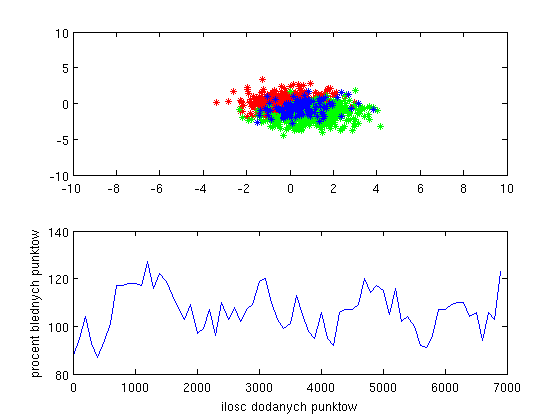
\includegraphics[width=\textwidth]{test_h0_1.png}
    \caption{h = 0,1}
  \end{subfigure}
  
  \begin{center}
  \begin{subfigure}[b]{0.5\textwidth}
    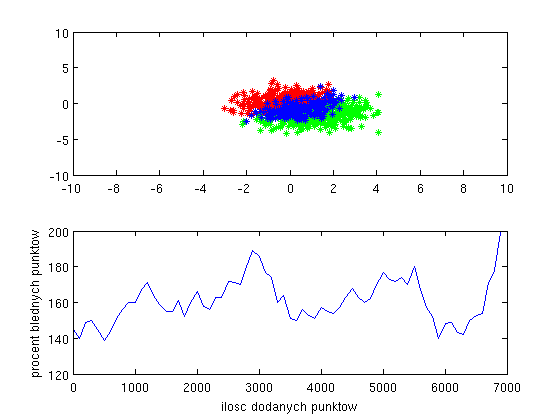
\includegraphics[width=\textwidth]{test_h1.png}
    \caption{h = 1}
  \end{subfigure}
  \end{center}
  
  \caption{Poszczególne etapy generowania danych}
  \label{test_h}
  
\end{figure}

Tabela \ref{h_table} przedstawia średnie wyniki błędów dla poszczególnych wartości spread. 

\begin{table}[H]
\centering
\begin{tabular}{|c|c|}
\hline
spread & błąd \\
\hline
0,0001 & 50\%  \\
\hline
0,001 & 45\%  \\
\hline
0,01 & 25\%  \\
\hline
0,1 & 106\%  \\
\hline
1 & 160\%  \\
\hline
\end{tabular}
\caption{Zestawienie wyników testów dla stałych wartości spread.}
\label{h_table}
\end{table}
Następnie przeprowadzono symulację dla h - wartości spread liczonej automatycznie. 

\section{Podsumowanie}

\end{document}